% 2011 年上海卷（文科）第 7 题：圆锥主视图（等腰三角形，腰 3、3，底 2）。
% 来源 PDF：普通高考/2011/2011上海文.pdf，SHA-256 ce52f4e95fde8fcfa636f06906fd95c4e685dfbf2bf8e400d8e7cca44a298535。
% 原页：第 1 页（印刷页 699）第 1 栏中部。
% 重绘依据：原图为实线等腰三角形，顶点朝上；两腰内侧各标 3，底边下方居中标 2。
% 该图即圆锥的轴截面（主视图）：底边 2 为底面直径，腰 3 为母线，高为 sqrt(3^2-1^2)=2*sqrt2。
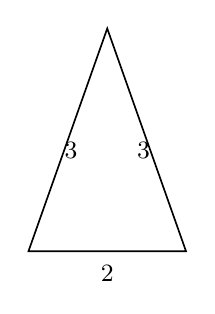
\begin{tikzpicture}[semithick, every node/.style={inner sep=1.5pt, font=\small}]
  \draw (0,2.828) -- (-1,0) -- (1,0) -- cycle;
  \node at (-0.46,1.28) {$3$};
  \node at (0.46,1.28) {$3$};
  \node at (0,-0.28) {$2$};
\end{tikzpicture}
